Quantum computing is to process quantum information by applying operations to it. As opposed to classical computers, quantum computers can make use of quantum phenomena, such as entanglement and superposition, to expedite calculations in some cases. To understand how to process information through a quantum computer it is essential to understand the mathematics of quantum computing.

\section{Basic Principles}
\subsection{Bra and ket notation}

A state vector

\begin{equation}
    \boldsymbol{x} = \begin{bmatrix} x_0 \\ x_1 \\ \vdots \\ x_{n-1} \\ x_n \end{bmatrix} \; ,
\end{equation}

is represented with the Dirac bra-ket notation as

\begin{equation}
    \boldsymbol{x} = \ket{x} = \begin{bmatrix} x_0\\ x_1 \\ x_2 \\ \dots \\ \dots \\ x_{n-1} \end{bmatrix} \; ,
\end{equation}

and the conjugate transpose

\begin{equation}
  \boldsymbol{x}^{\dagger} = \bra{x} = \begin{bmatrix} x_0^* & x_1^* & x_2^* & \dots & \dots & x_{n-1}^* \end{bmatrix} \; .
\end{equation}

With another state vector $\ket{y}$ we have the definition of the inner product

\begin{equation}
    \bra{y}\ket{x} = \sum_{i=0}^{n-1} y_i^*x_i=y_0^*x_0+y_1^*x_1+\dots + y_{n-1}^*x_{n-1} \; .
\end{equation}

and the outer product

\begin{equation}
    \ket{y}\bra{x} = \begin{bmatrix}
        y_{0}^*x_0 & y_{1}^*x_0 & \dots & y_{n-1}^*x_0 & y_{n}^*x_0 & \\y_{0}^*x_{1} & y_{1}^*x_{1} & \dots & y_{n-1}^*x_{1}  &  y_{n}^*x_{1} & \\ \vdots & \vdots & \ddots & \vdots & \vdots \\y_{0}^*x_{n-1} & y_{1}^*x_{n-1} & \dots & y_{n-1}^*x_{n-1} & y_{n}^*x_{n-1} & \\y_{0}^*x_{n} & y_{1}^*x_{n} & \dots & y_{n-1}^*x_{n} & y_{n}^*x_{n}
    \end{bmatrix}
\end{equation}

\subsection{The Qubit}

The most basic piece of information in quantum computing is the qubit, a quantum state with two different states. The standard orthonormal basis states of a qubit is as follows:

$$ \left | 0 \right > = \begin{bmatrix}
    1 \\ 0
\end{bmatrix} \; \space \; \left | 1 \right > = \begin{bmatrix}
    0 \\ 1
\end{bmatrix}$$

This means that the state can only be measured to be in state $\left | 0 \right >$ or $\left | 1 \right >$. Before measurement, however, the state of a qubit can be a superposition of the computational basis states. Which can be described as a linear combination of the two basis states:

$$\left | \psi \right > = \alpha \left | 0 \right > + \beta \left | 1 \right > = \begin{bmatrix}
    \alpha \\ \beta
\end{bmatrix}\; ,$$

where both $\alpha, \beta \in \mathbb{C}$ and with the normalization condition $\lvert\alpha\rvert + \lvert\beta\rvert = 1$. It is usefull to visualize the qubit as a sphere of possible states it can be in, called the Bloch sphere.

\begin{figure}[H]
    \centering
    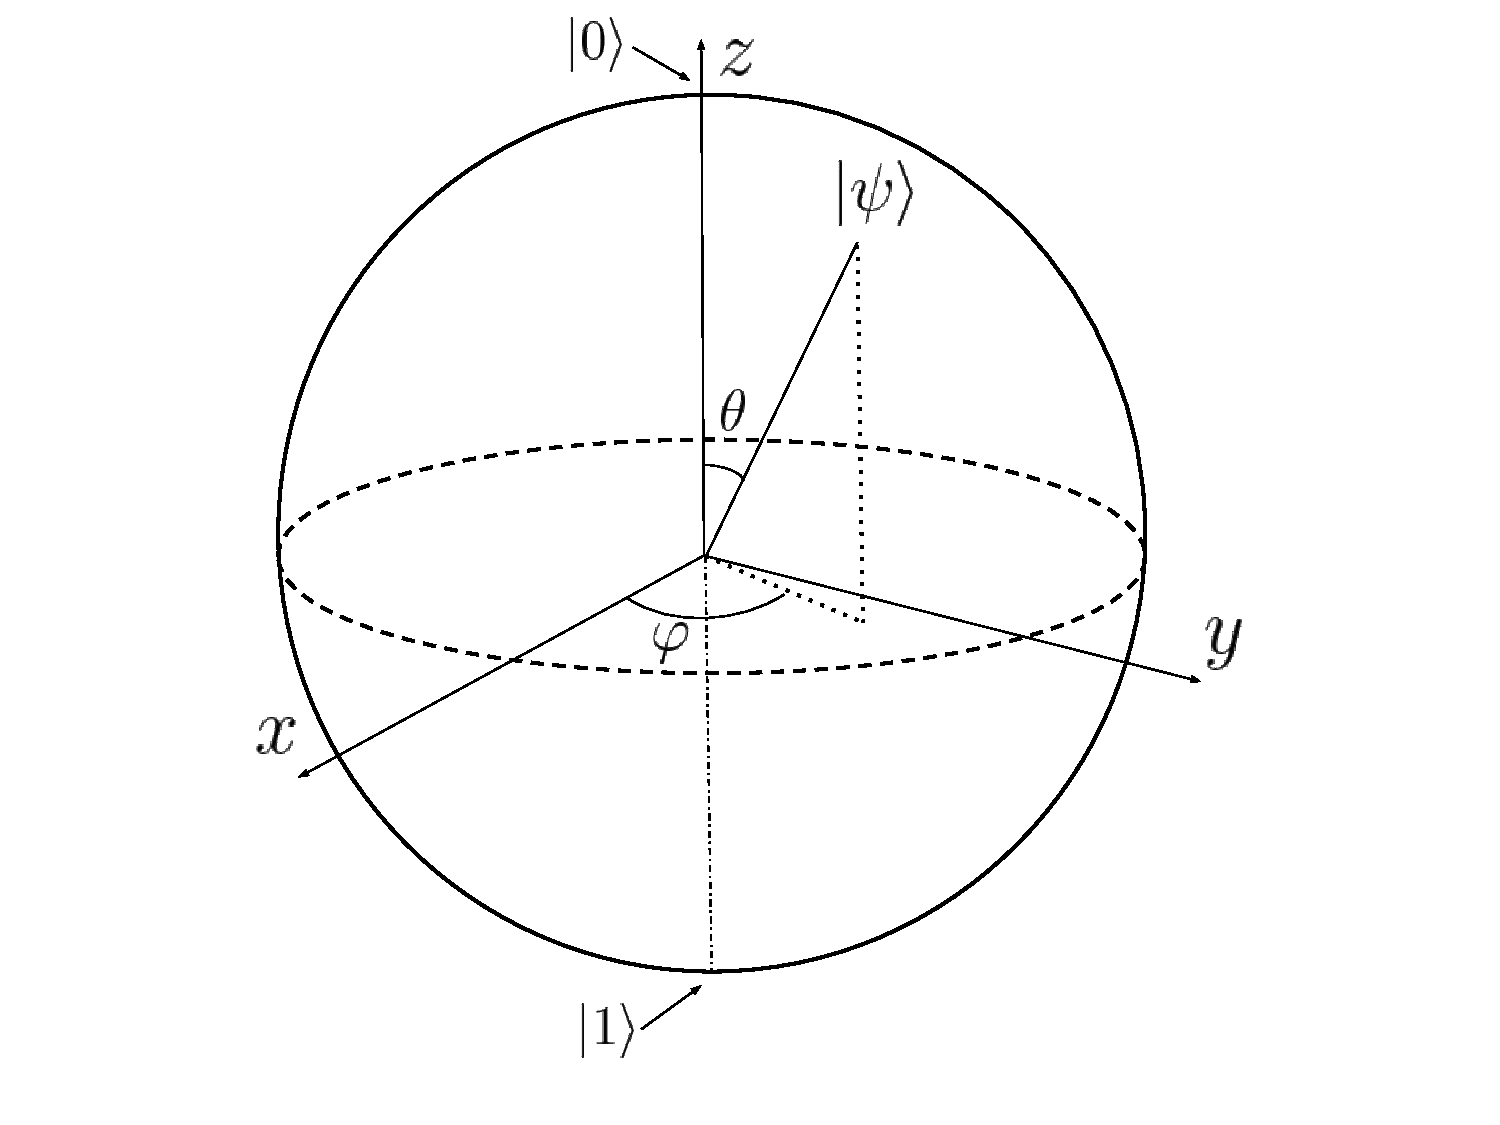
\includegraphics[width=\textwidth]{Figures/Drawn/bloch pshere.pdf}
    \caption{The possible states of a single qubit represented by a sphere with the apexes being the computational basis states.}
    \label{fig:blochsphere}
\end{figure}

Since we have the restriction $\lvert\alpha\rvert + \lvert\beta\rvert = 1$, the two complex values $\alpha$ and $\beta$ only contribute to two degrees of freedom, resulting in the surface of the Bloch sphere, \ref{fig:blochsphere}, as the state space of the single qubit. 
\subsection{Multi-Qubit States}

Bringing in another qubit will give us more possible measured outcomes. Therefor our computational basis needs to be expanded, encompassing every possible combination. This is done by tensor product of the possible single qubit measurements. For a two-qubit system we then have

\begin{gather}
\begin{aligned}\label{eq:twoqubit}
    \ket{0} \otimes \ket{0} = \begin{bmatrix} 1 \\ 0 \end{bmatrix} \otimes \begin{bmatrix} 1 \\ 0 \end{bmatrix} &=  \begin{bmatrix} 1 \\ 0 \\ 0 \\ 0\end{bmatrix} \\
    \ket{1} \otimes \ket{0} = \begin{bmatrix} 0 \\ 1 \end{bmatrix} \otimes \begin{bmatrix} 1 \\ 0 \end{bmatrix} &=  \begin{bmatrix} 0 \\ 1 \\ 0 \\ 0\end{bmatrix} \\
    \ket{0} \otimes \ket{1} = \begin{bmatrix} 1 \\ 0 \end{bmatrix} \otimes \begin{bmatrix} 0 \\ 1 \end{bmatrix} &=  \begin{bmatrix} 0 \\ 0 \\ 1 \\ 0\end{bmatrix} \\
    \ket{1} \otimes \ket{1} = \begin{bmatrix} 0 \\ 1 \end{bmatrix} \otimes \begin{bmatrix} 0 \\ 1 \end{bmatrix} &=  \begin{bmatrix} 0 \\ 0 \\ 0 \\ 1\end{bmatrix} \; ,  
\end{aligned}
\end{gather}
which then is a orthonormal basis for our new two-qubit system. To simplify writing, the tensorproduct between states are often written as

\begin{gather}
\begin{aligned}
    \ket{0} \otimes \ket{0} &= \ket{00} \\
    \ket{1} \otimes \ket{0} &= \ket{10} \\
    \ket{0} \otimes \ket{1} &= \ket{01} \\
    \ket{1} \otimes \ket{1} &= \ket{11} \; .
\end{aligned}
\end{gather}

Adding more qubits is simple. For each additonal qubit one tensormulitply the basis with the single-qubit basis, resulting in a $2^N$ possible measured states of the system. 
\subsection{Unitary Operators}

Unitary operators are used to transform a state to another. They are called unitary because of the condition:

\begin{equation}\label{eq:unitarydef}
    UU^* = U^*U = I \; ,
\end{equation}

where $I$ is the identity matrix of the same size as $U$. This condition is necessary such that the transformations doesn't change the size of the state vector. The unitary matrices applied to a state are often referred to as quantum gates, or just gates, as taken from logical gates in classical computing. For completeness we will give a explanation of all the gates used in this thesis:

The identity matrix does not transform a qubit, but it is an unitary matrix.

\begin{flalign}\label{eq:identity_matrix}
\textbf{Identity}\text{:} &&
 I = \begin{bmatrix}
        1 & 0 \\ 0 & 1
    \end{bmatrix}\; .&&
\end{flalign}

The Pauli spin matrices have applications outside of quantum computing and go by several different names, some which explain better what they do to a quantum bit. The first one is the

\begin{flalign}\label{eq:notgate}
\textbf{NOT Gate}\text{:} &&
 \sigma_x = \begin{bmatrix}
        0 & 1 \\ 1 & 0
    \end{bmatrix}\; ,&&
\end{flalign}

which rotates the state $\pi$ radians around the x-axis, also called bit flip gate because it flips $\left | 0 \right > $ to $\left | 1 \right >$. The

\begin{flalign}\label{eq:paulY}
\textbf{Pauli Y}\text{:} &&
 \sigma_y = \begin{bmatrix}
        0 & -i \\ i & 0
    \end{bmatrix}&&
\end{flalign}

rotates around the y-axis $\pi$ radians. While the

\begin{flalign}\label{eq:phaseflip}
\textbf{Phase Flip}\text{:} &&
 \sigma_y = \begin{bmatrix}
        1 & 0 \\ 0 & -1
    \end{bmatrix}&&
\end{flalign}

rotates around the z-axis $\pi$ radians. For transforming a state into a equal superposition of its opposite on the Bloch sphere we have the:

\begin{flalign}\label{eq:hadamardMatrix}
\textbf{Hadamard}\text{:} &&
    H = \frac{1}{\sqrt{2}}\begin{bmatrix}
        1 & 1 \\ 1 & -1
    \end{bmatrix} \; ,&&
\end{flalign}

which characteristically creates the equal superpositions from the base states:
\begin{alignat}{3}
H \left | 0 \right > = \frac{\left | 0 \right > + \left | 1 \right >}{\sqrt{2}} &
\quad \text{and} \quad &
H \left | 1 \right > = \frac{\left | 0 \right > - \left | 1 \right >}{\sqrt{2}} \; .
\end{alignat}

We also have the
\begin{flalign}\label{eq:phase_gate}
\textbf{Phase Gate}\text{:} &&
 S = \sqrt{\sigma_z} = \begin{bmatrix}
        1 & 0 \\ 0 & i
    \end{bmatrix}\; ,&&
\end{flalign}

which rotates the state $\frac{\pi}{2}$ radians around the z-axis. There are also gates which require a control, an additional qubit which changes the effect of the gate. An example is the

\begin{flalign}\label{eq:controlled_not}
\textbf{Controlled NOT}\text{:} &&
  \textbf{CNOT} = \begin{bmatrix}
        1 & 0 & 0 & 0 \\ 0 & 1 & 0 & 0 \\ 0 & 0 & 0 & 1 \\ 0 & 0 & 1 & 0 
    \end{bmatrix} \; ,&&
\end{flalign} 

which is essentially the identity when the control qubit is in state $\ket{0}$ and a \textbf{NOT} gate when the control qubit is in state $\ket{1}$. Then we have the

\begin{flalign}\label{eq:swap_gate}
\textbf{SWAP Gate}\text{:} &&
  \textbf{SWAP} = \begin{bmatrix}
        1 & 0 & 0 & 0 \\ 0 & 0 & 1 & 0 \\ 0 & 1 & 0 & 0 \\ 0 & 0 & 0 & 1 
    \end{bmatrix}\; ,&&
\end{flalign}

which switches the values of two target qubit.

\section{Quantum programming}

Quantum programming is setting up operations on quantum states in a specific order.

\subsection{Quantum Circuit}

To represent the operations done, their order and target states, one uses a quantum circuit. A single state, without any operations, in quantum circuit notation looks like the following

\begin{figure}[H]
    \centering
    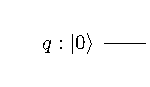
\includegraphics{Figures/Circuits/Theory/basecircuit.pdf}
\end{figure}

$q$ indicates in which bit of the registry the state resides and the line indicates what operations are done on the state, starting from left to right. So writing

$$H \ket{0}$$

in quantum circuit notation we have

\begin{figure}[H]
    \centering
    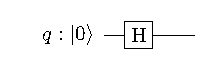
\includegraphics{Figures/Circuits/Theory/Hbasecircuit.pdf}
\end{figure}


Doing operations in a row, for example

$$\sigma_x  \sigma_yH \ket{0} \; ,$$

would be added to the right of the first Hadamard gate:

\begin{figure}[H]
    \centering
    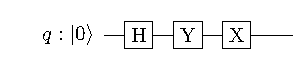
\includegraphics{Figures/Circuits/Theory/xyHbasecircuit.pdf}
\end{figure}

Some operations require a control. For the $\textbf{CNOT}$ gate we have the control marked by a $\Huge{\cdot}$ and the target qubit marked by $\oplus$ as shown here:

\begin{figure}[H]
    \centering
    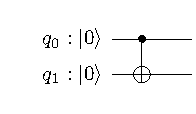
\includegraphics{Figures/Circuits/Theory/cxbasecircuit.pdf}
\end{figure}


\subsection{Measurement of Output}

In quantum mechanics we have that measuring a state changes it, or in our case the qubits collapses to either one of our base vectors $\ket{0}$ or $\ket{1}$. The measurement of a qubit on a quantum circuit is represented as the following:

\begin{figure}[H]
    \centering
    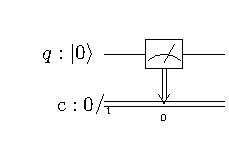
\includegraphics{Figures/Circuits/Theory/measurebasecircuit.pdf}
\end{figure}


Measuring here will either give us $\ket{0}$ or $\ket{1}$ with an equal $50\%$ chance. The information we want is most often the probabilities, and not the final state itself, since the probabilities ties to what state the qubit was in before it was measured. To extract the probabilities one utilizes the law of large numbers by computing the circuit a $N$ number of times and calculate the average number of $\ket{0}$ measurements and $\ket{1}$ measurements.

\subsection{Transformation of basis}

When measuring the qubits of a quantum circuit we are be often limited to doing the actual measuring in the z-basis. To overcome this limitation we simply transform the basis of the qubits to the basis we want to measure them in, or rather shift them back to the z-basis from the desired basis of measurement. The different basis transformations are as follows. \newline
\vskip 0cm
\textbf{Z-basis}:

\begin{figure}[H]
    \centering
    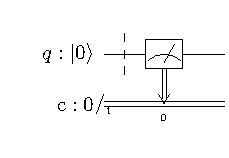
\includegraphics{Figures/Circuits/Theory/zm.pdf}
\end{figure}

Since we are already in the z-basis this one requires no transformation. The dashed line is to indicate that there are some sequence preceding it.
\newline\vskip 0cm
\textbf{X-basis}:

\begin{figure}[H]
    \centering
    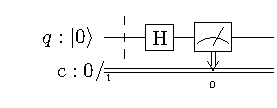
\includegraphics{Figures/Circuits/Theory/xm.pdf}
\end{figure}

which comes from the fact that

\begin{equation}
    HXH = Z \; .
\end{equation}

And similarly
\newline\vskip 0cm
\textbf{Y-basis}:

\begin{figure}[H]
    \centering
    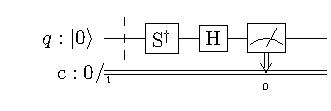
\includegraphics{Figures/Circuits/Theory/ym.pdf}
\end{figure}

where

\begin{equation}
    S^{\dagger}HYHS^{\dagger} = Z \; .
\end{equation}

\subsection{Circuit measurement to expectation value}

In the context of measurement the energy of a state for a given Hamiltonian we need to take into account the eigenvalues of the basis we measure in, here the z-basis. For the z-basis we have that

\begin{equation}
    Z\ket{0} = 1\ket{0} \;\;\;\;\;\;Z\ket{1} = -1\ket{1} \;,
\end{equation}

which means that for an example Hamiltonian

\begin{equation}
H_{\psi} = \varepsilon\sigma_x
\end{equation}

will have the expectation value

\begin{equation}
\left < H_{\psi} \right > = \varepsilon \left < \sigma_x \right > \; ,
\end{equation}

where

\begin{equation}
\left < \sigma_x \right > = n_0 - n_1 \; ,
\end{equation}

since we have matched it against the z-basis we measure in. Here $n_0$ and $n_1$ is the number of $\ket{0}$ and $\ket{1}$ measured respectively. For more than one qubit the eigenvalues accumulate. If we change our Hamiltonian to

\begin{equation}
H_{\psi} = \varepsilon\sigma_x \otimes \sigma_y \; ,
\end{equation}

we end up with the calculation of the expectation value

\begin{equation}
\left < \sigma_{x} \otimes \sigma_y \right > = n_{00} - n_{01} - n_{10} + n_{11}\; ,
\end{equation}

which can be generalized for $d\cdot n_s$ where $s$ is a basis state:

\begin{equation}
    d = (-1)^{N_1} \; ,
\end{equation}

where $N_1$ is the number of $1$'s in the basis state $s$.

\section{Entangled Qubits and Bell states}

\subsection{Entanglement}


To make two qubits entangled we need to make them dependent on each other, meaning that measuring one of the qubits gives us information about the output of the other. An intuitive approach would be to use a controlled gate, since the effect of the gate on the target qubit changes based on the state of the control qubit.
We start with two qubits in the $\ket{0}$ state.

\begin{equation}
    \begin{array}{cc}
        \textbf{Quantum Circuit:}  & \textbf{State after applied gates:} \\
        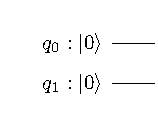
\includegraphics[scale=1.5, valign=c]{Figures/Circuits/Theory/2zero.pdf} &  \ket{q_1 q_2} = \ket{00} \; .
    \end{array}
\end{equation}

Then to put both qubit in a superposition we apply the Hadamard gate to each of them:

\begin{equation}\label{eq:2hadamard}
    \begin{array}{cc}
        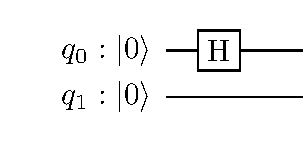
\includegraphics[valign=c]{Figures/Circuits/Theory/2hadamard.pdf} &  \ket{q_1 q_2} = \frac{\sqrt{2}}{2} |00\rangle+\frac{\sqrt{2}}{2} |10\rangle \; .
    \end{array}
\end{equation}


In doing so the first qubit becomes maximally mixed, meaning the first qubit is equally likely to be measured either $\ket{0}$ or $\ket{1}$, as seen in \ref{eq:2hadamard}. Still, the second qubit stays unchanged at $\ket{0}$, so measuring one of the qubits in \ref{eq:2hadamard} would not give us any information about the other. We apply then a \textbf{CNOT} gate:

\begin{equation}\label{eq:Bell1}
    \begin{array}{cc}
        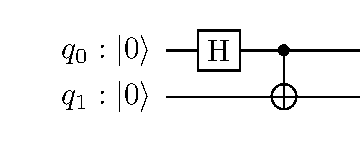
\includegraphics[valign=c]{Figures/Circuits/Theory/HadaCNOT.pdf} &  \ket{q_1 q_2} = \frac{\sqrt{2}}{2} |00\rangle+\frac{\sqrt{2}}{2} |11\rangle \; .
    \end{array}
\end{equation}

The \textbf{CNOT} gate makes it so that measuring $q_0 = \ket{0}$ tells us that $q_1 = \ket{0}$, while measuring $q_0 = \ket{1}$ makes it guaranteed that $q_1 = \ket{1}$, and vice versa. These linked measured values is what constitutes an entanglement of qubits.

\subsection{Bell States}

The resolving entangled state \ref{eq:Bell1} is one of the four maximally entangled states of a two-qubit system called the Bell states. There are four of them because of the four combination of initial states our two-qubit system can be in. We have the first one with initial state $\ket{00}$:

\begin{equation}\label{eq:00Bell}
    \begin{array}{cc}
        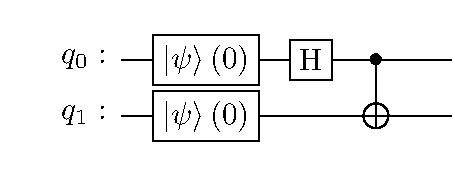
\includegraphics[scale=0.9, valign=c]{Figures/Circuits/Theory/00Bell.pdf} &  \ket{\Phi^+} = \frac{\sqrt{2}}{2} |00\rangle+\frac{\sqrt{2}}{2} |11\rangle \; .
    \end{array}
\end{equation}

For initial state $\ket{10}$:

\begin{equation}\label{eq:10Bell}
    \begin{array}{cc}
        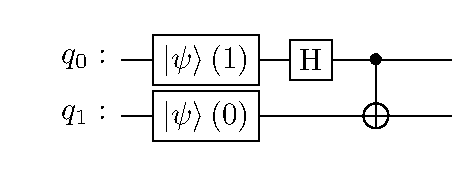
\includegraphics[scale=0.9, valign=c]{Figures/Circuits/Theory/10Bell.pdf} &  \ket{\Phi^-} = \frac{\sqrt{2}}{2} |00\rangle-\frac{\sqrt{2}}{2} |11\rangle \; .
    \end{array}
\end{equation}

And for $\ket{01}$

\begin{equation}\label{eq:01Bell}
    \begin{array}{cc}
        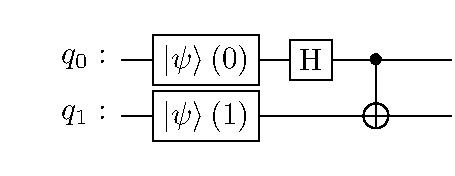
\includegraphics[scale=0.9, valign=c]{Figures/Circuits/Theory/01Bell.pdf} &  \ket{\Psi^+} = \frac{\sqrt{2}}{2} |10\rangle+\frac{\sqrt{2}}{2} |01\rangle \; .
    \end{array}
\end{equation}

And lastly $\ket{11}$:

\begin{equation}\label{eq:11Bell}
    \begin{array}{cc}
        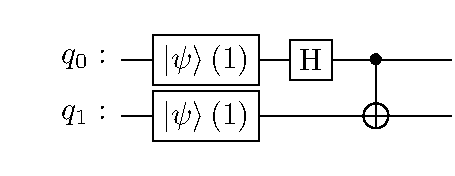
\includegraphics[scale=0.9, valign=c]{Figures/Circuits/Theory/11Bell.pdf} &  \ket{\Psi^-} = \frac{\sqrt{2}}{2} |10\rangle-\frac{\sqrt{2}}{2} |01\rangle \; .
    \end{array}
\end{equation}
\section{Noisy intermediate-scale Quantum}

The state of modern day quantum computers are in the so called 'noisy intermediate-scale quantum', meaning that the computers are not quite so accurate and with relatively few qubits. Taking into account, and minimizing, noise in our output is relevant when using real world quantum computers, opposed to simulated ones. 


\section{Variational Quantum Eigensolver}

Essentially the Varitonal Quantum Eigensolver, abrivated VQE, is a method to find the ground state of a Hamiltonian by variation of the state the system is in. Starting with a Hamiltonian in Pauli form:

\begin{equation}
\op{H} = \sum_i c_i \op{P}{i} \;
\end{equation}
where $c_i$ is the coefficient of the Pauli operator $\op{P}{i}$. We then have a general state $\ket{\psi}$ which is dependent on the angle to the z-axis, see \ref{fig:blochsphere}, for each qubit in the system.

\begin{equation}
   \ket{\psi \left ( \theta_1, \dots, \theta_N \right )} = \ket{\psi \left ( \boldsymbol{\theta} \right )} \; .
\end{equation}

Then the energy of that state is the expectation value

\begin{equation}
    E\left ( \boldsymbol{\theta} \right ) = \left < \op{H} \right > = \bra{\psi \left ( \boldsymbol{\theta} \right )} c_i \op{P}{i} \ket{\psi \left ( \boldsymbol{\theta} \right )} = \sum_i c_i \bra{\psi \left ( \boldsymbol{\theta} \right )} \op{P}{i} \ket{\psi \left ( \boldsymbol{\theta} \right )} \; .
\end{equation}

By variating the angles of $\boldsymbol{\theta}$ and checking the energy of each state we can then find the lowest energy state, which would then be the ground state of the system. Going through an exhaustive list of states would be extremely taxing computationally, especially with higher number of qubits. And in this case we shall see that it is unnecessary.

\subsection{Optimizing the choice of state}

